\documentclass[conference]{IEEEtran}
\IEEEoverridecommandlockouts

\usepackage{cite}
\usepackage{amsmath,amssymb,amsfonts}
\usepackage{algorithmic}
\usepackage{graphicx}
\usepackage{textcomp}
\usepackage{xcolor}
\usepackage{url}
\usepackage{array}
\usepackage{booktabs}
\usepackage{tabularx} % Added for automatic column width calculation
\usepackage{tikz}
\usetikzlibrary{arrows.meta,positioning,shapes.geometric}
\newcolumntype{Y}{>{\centering\arraybackslash}X}
\newcolumntype{P}[1]{>{\centering\arraybackslash}p{#1}}
\setlength{\tabcolsep}{3.5pt}
\renewcommand{\arraystretch}{1.0}
\setlength{\textfloatsep}{4pt plus 1pt minus 1pt}
\setlength{\floatsep}{3pt plus 1pt minus 1pt}
\setlength{\intextsep}{4pt plus 1pt minus 1pt}
\setlength{\dbltextfloatsep}{4pt plus 1pt minus 1pt}

\def\BibTeX{{\rm B\kern-.05em{\sc i\kern-.025em b}\kern-.08em
    T\kern-.1667em\lower.7ex\hbox{E}\kern-.125emX}}

\begin{document}

\title{Resource-Aware Adaptive Scheduling for Online Code Judge Systems}

\makeatletter
\newcommand{\linebreakand}{%
  \end{@IEEEauthorhalign}
  \hfill\mbox{}\par
  \mbox{}\hfill\begin{@IEEEauthorhalign}
}
\makeatother

\author{
\IEEEauthorblockN{Bharath Aashish R}
\IEEEauthorblockA{\textit{Dept. of Computer Science \& Engineering} \\
\textit{Easwari Engineering College}\\
Chennai, India \\
bharathaashish@gmail.com}
\and
\IEEEauthorblockN{Dhanush M}
\IEEEauthorblockA{\textit{Dept. of Computer Science \& Engineering} \\
\textit{Easwari Engineering College}\\
Chennai, India \\
dhanush.m.0808@gmail.com}
\linebreakand
\IEEEauthorblockN{Hemanthkumar K}
\IEEEauthorblockA{\textit{Dept. of Computer Science \& Engineering} \\
\textit{Easwari Engineering College}\\
Chennai, India \\
hemanthkumar2k04@gmail.com}
\and
\IEEEauthorblockN{Iniyaa P}
\IEEEauthorblockA{\textit{Dept. of Computer Science \& Engineering} \\
\textit{Easwari Engineering College}\\
Chennai, India \\
iniyaapaari@gmail.com}
\and
\IEEEauthorblockN{Indumathy P}
\IEEEauthorblockA{\textit{Assistant Professor, Dept. of CSE} \\
\textit{Easwari Engineering College}\\
Chennai, India \\
indumathy.p@eec.srmrmp.edu.in}
}
\maketitle

\begin{abstract}
Online Code Judge (OJ) systems often assign every submission a fixed worst-case resource limit, such as 2048~MiB of RAM and 2.0 CPU cores. We deployed our judge on Google Cloud Platform (an \texttt{e2-standard-4} instance in \texttt{asia-south1}) and measured 399 accepted submissions executing at the 256~MiB tier: 96.2\% used less than 25~MiB of resident set size (RSS), with a median of 5.7~MiB, and every submission completed inside Tier~1 without requiring promotion. We present RAAS-OCJS, a resource-aware scheduling framework that combines Linux cgroups~v2 with tiered allocation and AST-based XGBoost routing. Kernel-level profiles across C++, Python, Java, and C programs, spanning light, medium, and memory-heavy submissions, were used to drive a 10,000-submission contest simulation. Compared with static allocation, watermark-driven reactive promotion reduced reserved RAM by 81.49\% and CPU core-hours by 47.93\%, while allocating independent Tier~2 capacity on prediction alone reached only 27.85\%, because it charges predicted-heavy submissions at the worst-case ceiling rather than discovering actual need. In a simulated 500-submission freeze rush, queue wait fell from 73,134.0~ms to zero and burst drain time from 182.6~s to 34.0~s, while P95 turnaround fell from 144,649.9~ms to 4,491.7~ms. A 19-case promotion stress suite confirms the mechanism directly: submissions demanding 400~MiB exceed the 256~MiB tier in both Python and C++ with zero kernel OOM kills, and the watermark triggers exactly at its configured 179.2~MiB threshold. A 128~MiB boundary experiment additionally isolates three independent failure modes, which together establish 256~MiB as the practical minimum tier. These results support adaptive resource allocation for improving judge-system utilization and concurrency.
\end{abstract}

\begin{IEEEkeywords}
Online judge systems, resource-aware scheduling, adaptive cgroups, soft watermark, AST analysis, XGBoost, cloud provisioning, queue latency.
\end{IEEEkeywords}

\section{Introduction}
Online code judge (OJ) platforms underpin computer science education, competitive programming contests (such as the International Collegiate Programming Contest, ICPC), and automated technical interviews \cite{wasik2018survey}. As programming education expands, judges must evaluate thousands of code submissions concurrently while guaranteeing deterministic isolation and strict sandboxing. Existing research has addressed this computational demand primarily through infrastructure-level expansion: deploying elastic cloud clusters \cite{pan2022cloud}, distributing jobs over message queues \cite{song2025idl}, or deploying geographically replicated edge judges \cite{wang2021metaoj}.

These approaches share a fundamental, costly assumption: \textit{every submission, regardless of its computational structure, receives identical, worst-case sandbox resource ceilings} (typically 2048~MiB of RAM and 2.0 CPU cores).

This convention creates three practical problems:
\begin{itemize}
    \item \textbf{Resource Underutilization}: Most contest submissions implement standard algorithmic logic (e.g., prefix sums, two pointers, greedy string scans), and in our measurements these typically required 5~MiB to 25~MiB of resident set size (RSS), with 96.2\% of accepted runs below 25~MiB and a median of 5.7~MiB (Table~\ref{tab:mem_dist}). Reserving 2048~MiB for each of them leaves most of that allocation idle.
    \item \textbf{Concurrency Starvation on Fixed Hardware}: In air-gapped regional contests or campus lab servers, where external cloud bursting is not an option, the judge runs on a fixed physical machine (e.g., 15~GiB usable RAM). A static 2048~MiB quota limits concurrency to 7 execution slots on that host, which produces queue backlogs and submission timeouts during a scoreboard freeze rush.
    \item \textbf{Cloud Billing Inflation}: Public cloud providers bill by reserved node capacity, not actual usage. Provisioning for the worst case means contest organizers end up renting far more virtual machines than the workload actually needs: our deployment on Google Cloud Platform (Section~\ref{sec:cloud}) shows that a 500-submission freeze rush requires 72 conventionally-provisioned instances where 9 suffice, an 8.0$\times$ over-provisioning.
\end{itemize}

To address this, this paper presents \textbf{RAAS-OCJS} (Resource-Aware Adaptive Scheduling for Online Contest Judge Systems), which introduces a two-tier execution framework:
\begin{enumerate}
    \item A lightweight default sandbox (\textbf{Tier 1: 256~MiB RAM, 1.0 CPU core}) that completed all 399 measured submissions on our cloud deployment without a single promotion;
    \item An active Linux cgroup~v2 soft watermark ($\theta = 70\%$, corresponding to 179.2~MiB) that detects high memory utilization in-flight and lifts the container's memory and CPU limits to \emph{uncapped} mid-execution, without restarting the container or losing process state. Measured from submission acceptance to completed promotion this takes 610--913~ms when the workload reaches the watermark immediately, and 3.2--5.0~s when it ramps gradually, since the interval necessarily includes the time taken to reach the watermark (Section~\ref{sec:promotion_verify});
    \item An offline Machine Learning (XGBoost) classifier driven by Tree-sitter Abstract Syntax Tree (AST) static structural metrics that predicts memory-intensive jobs upon ingress.
\end{enumerate}



\section{Theoretical Model and Queueing Architecture}

\subsection{Mathematical Formulation of Memory Waste}
Let $S = \{s_1, s_2, \dots, s_N\}$ denote a sequence of $N$ submissions entering an online judge. Under static overprovisioning, the system assigns a fixed resource allocation:
\begin{equation}
R_{\mathrm{alloc}}(s_i) = R_{\mathrm{max}}, \quad \forall s_i \in S
\end{equation}
where $R_{\mathrm{max}}$ is typically 2048~MiB. Let $R_{\mathrm{peak}}(s_i)$ denote the actual peak resident set size (RSS) consumed by $s_i$. The unallocated, wasted memory for submission $s_i$ is:
\begin{equation}
\mathrm{Waste}(s_i) = R_{\mathrm{alloc}}(s_i) - R_{\mathrm{peak}}(s_i)
\end{equation}
The system-wide memory waste percentage $W$ across a contest of $N$ submissions is:
\begin{equation}
W = \left[ \frac{\sum_{i=1}^N \left( R_{\mathrm{alloc}}(s_i) - R_{\mathrm{peak}}(s_i) \right)}{\sum_{i=1}^N R_{\mathrm{alloc}}(s_i)} \right] \times 100\%
\end{equation}
Because introductory and greedy problems require merely 6~MiB to 25~MiB, $R_{\mathrm{peak}}(s_i) \ll R_{\mathrm{max}}$. Our simulation of this waste model reports 98.83\% of allocated memory wasted under the static baseline.

\subsection{Concurrency Capacity and Queueing Collapse}
On a host with usable physical RAM $M_{\mathrm{host}}$ and operating system reserve $M_{\mathrm{os}}$, the safe concurrency capacity $K$ under non-overcommitted execution is:
\begin{equation}
K_{\mathrm{safe}} = \left\lfloor \frac{M_{\mathrm{host}} - M_{\mathrm{os}}}{R_{\mathrm{alloc}}} \right\rfloor
\end{equation}
On our 15~GiB physical calibration host ($M_{\mathrm{host}} = 15,360$~MiB, $M_{\mathrm{os}} = 1,024$~MiB), baseline static allocation ($R_{\mathrm{max}} = 2048$~MiB) limits concurrency strictly to:
\begin{equation}
K_{\mathrm{safe, baseline}} = \left\lfloor \frac{15,360 - 1,024}{2048} \right\rfloor = 7 \text{ slots}
\end{equation}

We model contest submission arrival as a non-homogeneous Poisson process with time-varying arrival rate $\lambda(t)$. Service times follow a general distribution with mean $E[X] = 1/\mu$ and variance $\sigma^2$, constituting an $M/G/K$ queueing system.

During a freeze rush spike of 500 submissions in 30~s ($\lambda = 16.67$~submissions/s), against average service time $E[X] \approx 0.85$~s, the 7-slot baseline service capacity is $\mu = 7 / 0.85 \approx 8.24$~submissions/s. Because $\lambda > \mu$, queue backlogs explode immediately. Under RAAS-OCJS with $R_{\mathrm{light}} = 256$~MiB, concurrency expands safely to $\lfloor 14{,}336/256 \rfloor = 56$ slots (utilizing 93.3\% of host RAM as reserved capacity, which the watermark then releases in practice). At $K = 56$, $\mu = 56 / 0.85 \approx 65.88$~submissions/s, satisfying $\mu \gg \lambda$ and maintaining zero queue wait ($L_q \approx 0$).

\subsection{Dynamic Soft Watermark Governance}
RAAS-OCJS implements a two-tier scheduling policy:
\begin{itemize}
    \item \textbf{Tier 1 (Light Sandbox)}: $R_{\mathrm{light}} = 256$~MiB, 1.0 CPU core (1024 CFS shares).
    \item \textbf{Tier 2 (High Sandbox)}: unbounded, 2.0 CPU cores (2048 CFS shares). The 2048~MiB figure is the \emph{static baseline's} convention that we compare against, not a ceiling RAAS-OCJS re-imposes after promotion.
\end{itemize}
Rather than statically placing containers into Tier 2, all submissions enter Tier 1 by default. The judge daemon configures the Linux cgroups v2 controller with a soft memory watermark threshold $\theta = 0.70$:
\begin{equation}
\mathrm{Threshold}_{\mathrm{wm}} = \theta \times R_{\mathrm{light}} = 0.70 \times 256\text{ MiB} = 179.2\text{ MiB}
\end{equation}
When $R_{\mathrm{current}}(t) \ge \mathrm{Threshold}_{\mathrm{wm}}$, the kernel emits a pressure notification. The judge daemon then lifts the limits in parallel with process execution by writing \texttt{max} to the container's cgroup~v2 \texttt{memory.high} and \texttt{memory.max} files, raising both the memory ceiling and the CPU quota to uncapped without restarting the container. The kernel write is the entire promotion: it takes effect immediately and preserves process state. (An earlier implementation instead followed the cgroup write with \texttt{docker update -{}-memory 0 -{}-cpus 0}; that call is silently self-defeating, and Section~\ref{sec:promotion_verify} documents both the failure and its correction.) This leaves a 76.8~MiB safety cushion ($256 - 179.2$) so the update can complete before an OOM condition occurs. Promotion targets \emph{uncapped} rather than a fixed 2048~MiB tier: the watermark fires precisely when a submission has already shown that it outgrows Tier~1, and in our stress suite such submissions demanded 185~MB to 900~MB, so no single fixed ceiling is appropriate.

% System architecture overview
\begin{figure*}[!t]
\centering
\resizebox{0.86\textwidth}{!}{%
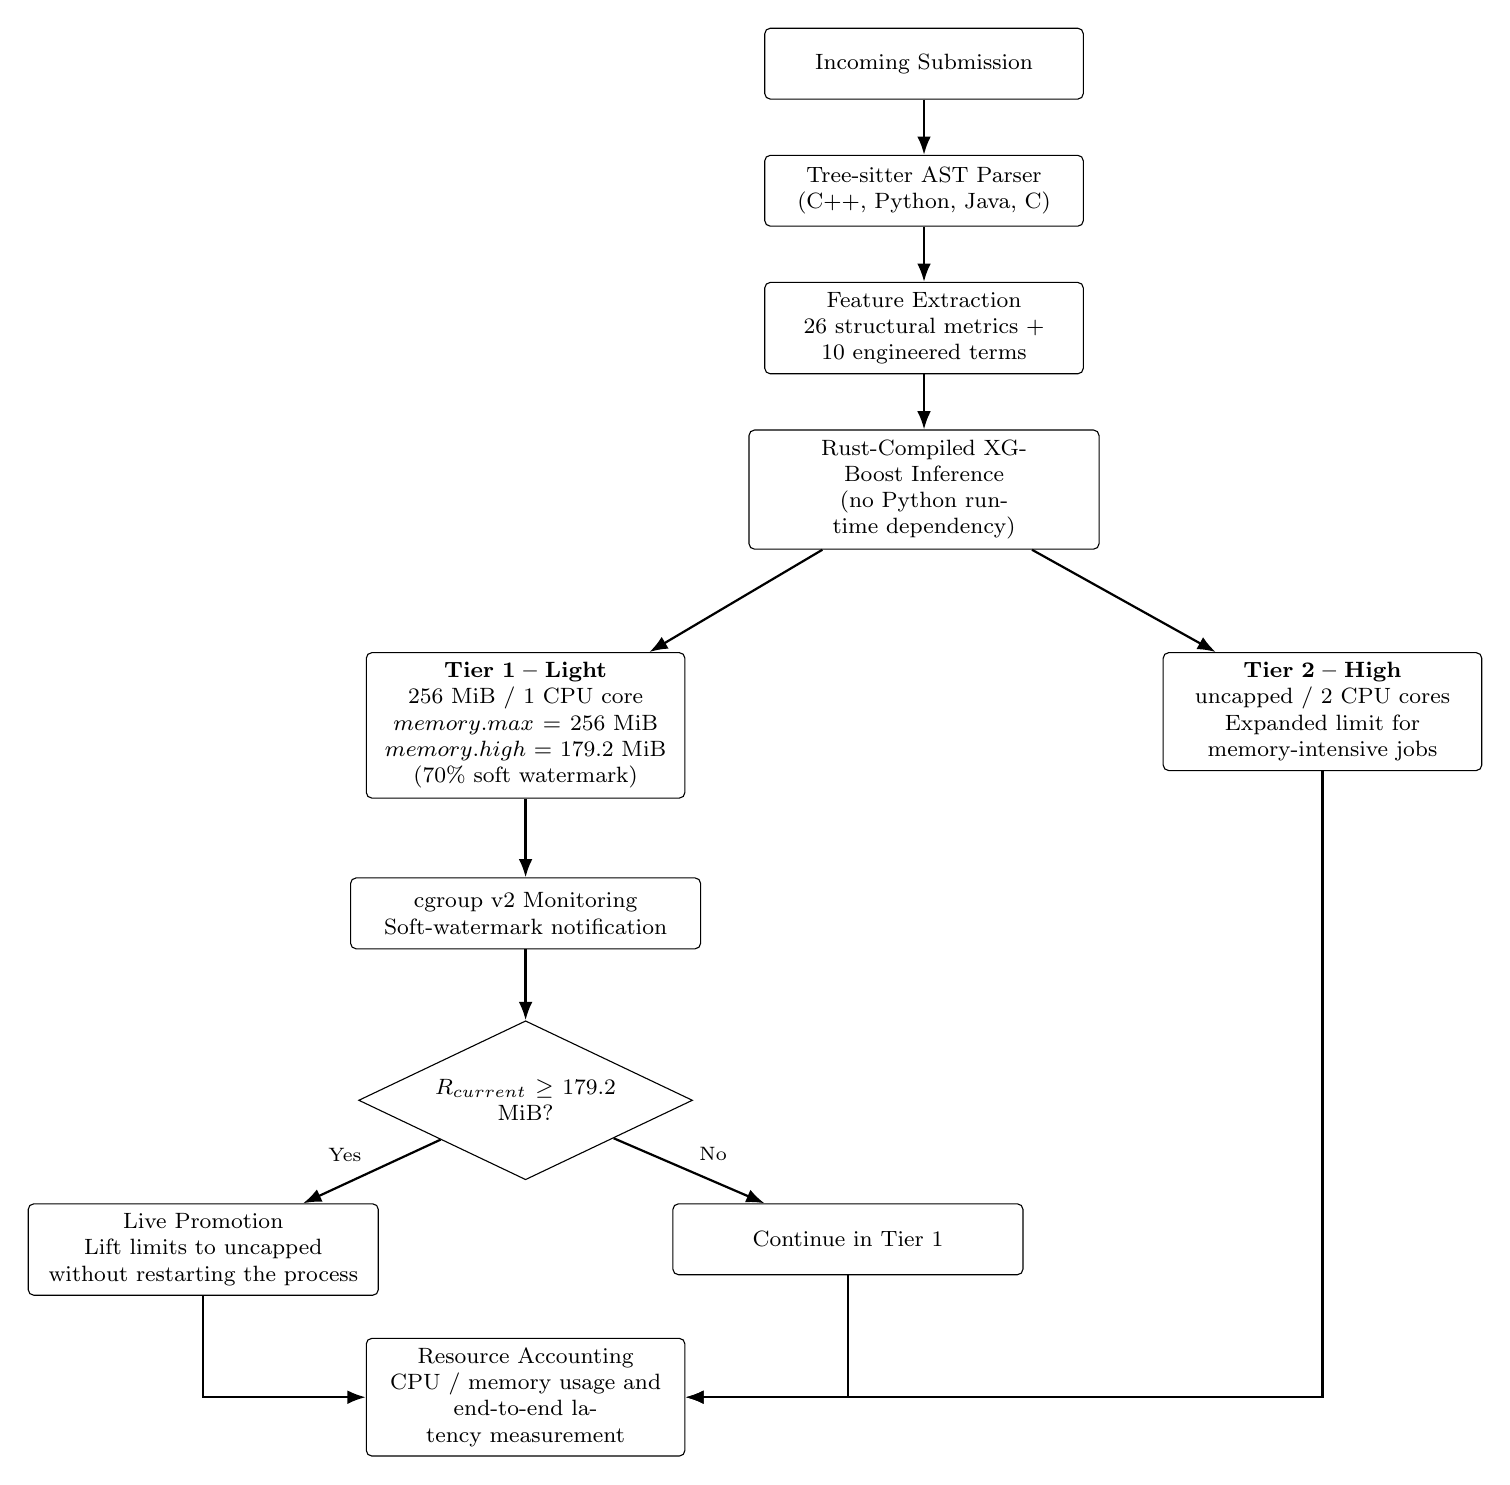
\begin{tikzpicture}[
    >=Latex,
    node distance=7mm and 16mm,
    block/.style={draw, rounded corners=2pt, align=center, minimum height=9mm, text width=38mm, inner sep=3.5pt, font=\footnotesize},
    smallblock/.style={draw, rounded corners=2pt, align=center, minimum height=9mm, text width=42mm, inner sep=3.5pt, font=\footnotesize},
    decision/.style={draw, diamond, aspect=2.1, align=center, inner sep=2pt, text width=27mm, font=\footnotesize},
    line/.style={-Latex, thick}
]
% Main processing pipeline: vertically stacked for a cleaner reading order.
\node[block] (input) {Incoming Submission};
\node[block, below=of input] (parser) {Tree-sitter AST Parser\\(C++, Python, Java, C)};
\node[block, below=of parser] (features) {Feature Extraction\\26 structural metrics +\\10 engineered terms};
\node[smallblock, below=of features] (model) {Rust-Compiled XGBoost Inference\\(no Python runtime dependency)};

% Initial resource tiers.
\node[block, below left=13mm and 8mm of model] (light) {\textbf{Tier 1 -- Light}\\256 MiB / 1 CPU core\\$memory.max=256$ MiB\\$memory.high=179.2$ MiB\\(70\% soft watermark)};
\node[block, below right=13mm and 8mm of model] (heavy) {\textbf{Tier 2 -- High}\\uncapped / 2 CPU cores\\Expanded limit for memory-intensive jobs};

% Reactive Tier 1 path.
\node[smallblock, below=10mm of light] (monitor) {cgroup v2 Monitoring\\Soft-watermark notification};
\node[decision, below=9mm of monitor] (decision) {$R_{current} \ge 179.2$ MiB?};
\node[smallblock, below left=8mm and 8mm of decision] (promote) {Live Promotion\\Lift limits to uncapped\\without restarting the process};
\node[smallblock, below right=8mm and 8mm of decision] (continue) {Continue in Tier 1};

% Final measurement stage centered beneath both branches.
\node[block, below=20mm of decision] (account) {Resource Accounting\\CPU / memory usage and\\end-to-end latency measurement};

% Main arrows.
\draw[line] (input) -- (parser);
\draw[line] (parser) -- (features);
\draw[line] (features) -- (model);
\draw[line] (model) -- (light);
\draw[line] (model) -- (heavy);
\draw[line] (light) -- (monitor);
\draw[line] (monitor) -- (decision);
\draw[line] (decision) -- node[above left, font=\scriptsize]{Yes} (promote);
\draw[line] (decision) -- node[above right, font=\scriptsize]{No} (continue);

% Cleanly route all execution paths into resource accounting.
\draw[line] (promote.south) |- (account.west);
\draw[line] (continue.south) |- (account.east);
\draw[line] (heavy.south) |- (account.east);

\end{tikzpicture}%
}
\caption{RAAS-OCJS execution and predictive tiering workflow. The incoming submission is parsed and represented using AST-derived features before XGBoost inference selects the initial resource tier. Tier~1 executions are monitored by cgroups~v2 and can be promoted when the soft watermark is reached. Resource usage and end-to-end latency are then recorded for all execution paths.}
\label{fig:raas_architecture}
\end{figure*}

\section{System Implementation and Methodology}

% MOVED TABLE: Placed here so it renders in Section IV


The evaluation testbed was implemented and calibrated on dedicated bare-metal hardware:
\begin{itemize}
    \item \textbf{Processor}: 13th Gen Intel Core i5-13420H (12 logical CPUs, 8 cores: 4 Performance cores up to 4.60 GHz + 4 Efficient cores up to 3.40 GHz).
    \item \textbf{Physical Memory}: 15 GiB usable DDR5 RAM.
    \item \textbf{Storage}: NVMe PCIe 4.0 Solid State Drive.
    \item \textbf{Operating System}: Fedora Linux (Kernel \texttt{7.1.3-201.fc44.x86\_64}).
    \item \textbf{Container Engine}: Docker Engine 29.8.1 with cgroupfs driver on unified hierarchy (\texttt{/sys/fs/cgroup}).
\end{itemize}



\subsection{Real Dataset Selection}
Our primary measurement is a cloud run: 399 submissions accepted and executed live against the deployed judge at the shipped 256~MiB tier, across three languages, drawn from the Hugging Face \texttt{deepmind/code\_contests} \cite{li2022alphacode} dataset. All 399 returned \texttt{AC} inside Tier~1 and none required promotion. Because CodeContests is crowd-sourced, we do not take the first solution offered for a language: each candidate is first executed against the problem's own public test, and only the first candidate returning \texttt{AC} is kept. These 399 measured profiles are the corpus the 10,000-submission and 500-submission simulations sample from (Section~IV-B, IV-C); those larger scenarios were not executed as 10,000 or 500 separate live container runs.

That cloud corpus is a faithful sample of ordinary contest traffic but it contains no memory-heavy submissions at all --- its maximum peak is 47.8~MiB, far below the 179.2~MiB watermark --- so on its own it cannot exercise promotion. To represent the heavy tail we draw on an earlier bare-metal calibration: 72 live container evaluations across C++20 (\texttt{g++ 14.2}), Python 3.12, Java 17 (OpenJDK HotSpot), and C17 (\texttt{gcc 14.2}), drawn from \texttt{code\_contests} and \texttt{CodeNet} \cite{puri2021codenet}. That set contains the two-dimensional knapsack family, whose cells peak at 204--254~MiB and sit above the watermark. It yields 69 \texttt{AC} of 72 at 256~MiB, the three exceptions being Java on the memory-heavy problem, identified in Section~\ref{sec:boundary}. The simulations therefore sample a combined corpus: the 399 cloud-measured profiles, plus the heavy and medium profiles from this calibration, with the heavy family deliberately oversampled at a 20\% stress rate so that promotion and its reservation cost are exercised rather than assumed away. We report the combination explicitly because it changes the result: on the cloud-measured submissions alone the Reactive strategy saves 87.4\% of reserved memory, whereas the heavy-inclusive corpus below reports 81.49\%.

The two corpora also differ in shape, and the difference is the point of the paper. In the cloud corpus the mean is 10.7~MiB against a median of 5.7~MiB; 96.2\% of runs sit below 25~MiB, and the maximum is 47.8~MiB. In the bare-metal calibration, four memory-heavy cells at 204--254~MiB pull the mean to 49.2~MiB against a median of 13.4~MiB. Both distributions are bimodal rather than merely skewed --- most submissions sit an order of magnitude below the ceiling while a small number approach it --- and summarising either with a single mean conceals exactly the spread that motivates adaptive tiering.

\begin{table}[!t]
\caption{Resident Memory Used by the 399 Cloud-Measured Submissions (256 MiB Tier, All AC)}
\label{tab:mem_dist}
\centering
\scriptsize
\begin{tabular}{|l|c|c|c|c|c|}
\hline
\textbf{Language} & \textbf{Runs} & \textbf{$<$25 MiB} & \textbf{Median} & \textbf{Mean} & \textbf{Max} \\
\hline
C++ & 168 & 95.2\% & 5.6 MB & 7.9 MB & 47.8 MB \\
\hline
Python & 119 & 100.0\% & 5.2 MB & 6.1 MB & 13.1 MB \\
\hline
Java & 112 & 93.8\% & 19.3 MB & 19.6 MB & 36.8 MB \\
\hline
\textbf{All} & \textbf{399} & \textbf{96.2\%} & \textbf{5.7 MB} & \textbf{10.7 MB} & \textbf{47.8 MB} \\
\hline
\end{tabular}
\end{table}



\subsection{AST Feature Extraction and XGBoost Predictive Tiering}
Before launching an execution container, RAAS-OCJS can optionally run a static code analysis pass to predict whether an incoming submission fits safely within Tier~1 (256~MiB) or should be provisioned directly with Tier~2 (uncapped). This predictive stage couples a Tree-sitter Abstract Syntax Tree (AST) feature extractor with in-process XGBoost classifiers \cite{chen2016xgboost}.

\textit{1) Static AST Feature Extraction:} Using language-specific Tree-sitter grammars compiled directly into our Rust daemon, the extractor parses source code into a concrete syntax tree in under 1.5~ms. In a single linear traversal of the tree, it computes 26 structural metrics:
\begin{itemize}
    \item \textbf{Control Flow and Loops}: Maximum block nesting depth, deepest loop nesting depth (which correlates with polynomial execution complexity $O(N^k)$), total loop statements, and McCabe cyclomatic complexity.
    \item \textbf{Recursion Topology}: A binary recursion flag and self-call site count, which differentiate simple linear recursion $O(N)$ from exponential divide-and-conquer or backtracking branching $O(2^N)$.
    \item \textbf{Memory and Container Patterns}: Detection of explicit large heap/BSS allocations ($\ge 10^6$ elements or bytes, such as \texttt{malloc}, \texttt{new int[]}, container sizing, or large static arrays) as a single boolean, complemented by four \emph{measured} allocation aggregates: the largest and summed statically-known allocation size, the number of recognised allocation sites, and the number of sites whose size is only known at runtime; high-throughput I/O patterns (\texttt{sync\_with\_stdio}, \texttt{BufferedReader}, \texttt{sys.stdin.readline}), and standard library collections known for memory overhead (\texttt{unordered\_map}, \texttt{priority\_queue}, \texttt{BigInteger}, \texttt{defaultdict}).
    \item \textbf{Scale and Access Topology}: Total array/collection subscript expressions (\texttt{a[i]}), chained multi-dimensional indexing (\texttt{grid[i][j]} for 2D dynamic programming tables or graph adjacency matrices), function count, call sites, total AST node count, maximum tree depth, and source lines of code (SLOC).
\end{itemize}
From these 26 raw counts, the pipeline derives 10 interaction and scale terms: four density ratios normalised by AST size, source length, or function count (loop, call, subscript, and arithmetic density), a 2D subscript ratio, a recursion-intensity term, a log-scaled maximum integer constant, and log-scaled AST node and source character counts. The maximum-integer-constant term is a weaker allocation signal than its earlier description implied: it records the largest literal \emph{token}, so \texttt{new byte[200 << 20]} contributes $200$ and \texttt{new byte[200*1024*1024]} contributes $1024$, not the evaluated size. Allocation magnitude is instead captured directly by the four measured aggregates listed above: \texttt{alloc\_size\_max} and \texttt{alloc\_size\_total} (largest and summed statically-known size), \texttt{alloc\_sites} (count of recognised sites) and \texttt{alloc\_unknown\_sites} (sites whose size is only known at runtime, such as \texttt{malloc(n)} or \texttt{new byte[chunks]}). The two size fields are language-relative rather than byte-denominated --- C \texttt{malloc} sizes are bytes, whereas Java and Python \texttt{new T[n]} sizes are element counts --- so the fields are deliberately named \texttt{size} rather than \texttt{bytes}. This yields a 36-dimensional vector for the specialized per-language models, or 40 features for the unified model, which appends four one-hot language encodings.

\textit{2) Model Training and Validation:}
We trained gradient-boosted decision trees using XGBoost (\texttt{tree\_method='hist'}, $n_{\mathrm{estimators}} = 250$, learning rate $\eta = 0.04$, max tree depth $d = 6$, minimum child weight $2$, subsample ratio $0.85$, column subsample $0.85$, $\gamma = 0.1$, $L_1$ penalty $\alpha = 0.05$, and $L_2$ penalty $\lambda = 1.0$). Because contest submissions are heavily skewed toward lightweight solutions, we applied class re-weighting using $\texttt{scale\_pos\_weight} = N_{\mathrm{light}} / N_{\mathrm{heavy}}$ during training.

To avoid data leakage across submissions for the same problem, we evaluated the models with 5-fold \textbf{Problem-Grouped Cross-Validation} (\texttt{GroupKFold} grouped strictly by \texttt{problem\_id}). Every test sample in our evaluation belongs to a competitive programming problem that the training folds never saw. In addition, rather than accepting a default $0.5$ decision threshold, we tuned the threshold $\tau$ for each language using Youden's $J$ statistic ($J = \mathrm{Sensitivity} + \mathrm{Specificity} - 1$) on validation folds to balance recall against false tier promotions.

\begin{table*}[!t]
\caption{XGBoost Model Performance on Unseen Contest Problems (Problem-Grouped Validation)}
\label{tab:ml_metrics}
\centering
\scriptsize
\begin{tabularx}{\textwidth}{|Y|Y|c|c|c|c|c|c|}
\hline
\textbf{Dataset Source} & \textbf{Model Architecture} & \shortstack{\textbf{5-Fold}\\\textbf{CV Acc.}} & \shortstack{\textbf{Test Acc.}\\\textbf{(Unseen)}} & \textbf{F1-Score} & \textbf{Precision} & \textbf{Recall} & \shortstack{\textbf{ROC-}\\\textbf{AUC}} \\
\hline
IBM Project CodeNet & Unified Multi-Language & 89.56\% & 87.38\% & 88.48\% & 85.21\% & 92.01\% & 0.9503 \\
(164,686 Submissions, & Specialized C++ Model & 96.07\% & 94.39\% & 96.26\% & 99.74\% & 93.02\% & 0.9904 \\
Measured-Memory Labels) & Specialized Java Model & 86.73\% & 84.19\% & 83.30\% & 79.01\% & 88.07\% & 0.9172 \\
& Specialized Python Model & 85.02\% & 83.71\% & 86.51\% & 90.01\% & 83.27\% & 0.9221 \\
& Specialized C Model\footnotemark[1] & 97.76\% & 96.64\% & 41.12\% & 27.85\% & 78.57\% & 0.9387 \\
\hline
DeepMind CodeContests & Unified Multi-Language & 84.73\% & 94.45\% & 92.03\% & 88.18\% & 96.22\% & 0.9886 \\
(30,000 Submissions, & Specialized C++ Model & 83.38\% & 95.45\% & 94.27\% & 91.59\% & 97.12\% & 0.9938 \\
Length-Heuristic Labels) & Specialized Java Model & 80.22\% & 82.82\% & 81.37\% & 74.62\% & 89.46\% & 0.9380 \\
& Specialized Python Model & 94.69\% & 98.88\% & 97.85\% & 96.38\% & 99.36\% & 0.9961 \\
\hline
\end{tabularx}
\end{table*}

\textit{3) Empirical Model Metrics on Unseen Problems:}
Table~\ref{tab:ml_metrics} summarizes performance on held-out, unseen contest problems across two corpora that differ in how the \emph{label} was obtained, and the distinction matters more than the headline figures. On IBM Project CodeNet the labels are \emph{measured} memory consumption, so the classifier is predicting the quantity the tiering decision actually depends on: 164,686 submissions spanning 2,520 unique problems, labelled Heavy at $\ge 100$~MiB of measured memory and Light below 25~MiB, with the ambiguous 25--100~MiB band dropped rather than guessed. There, the specialized C++ model reached a 94.39\% test accuracy, a 96.26\% F1-score and an ROC-AUC of 0.9904 on unseen problems, while the specialized Java and Python models reached 84.19\% and 83.71\% test accuracy (ROC-AUC 0.9172 and 0.9221). On DeepMind CodeContests the labels instead came from a source-length heuristic, and the same architectures score appreciably higher against that target (up to 98.88\% in Python). That gap is informative rather than flattering: correlation between source length and measured memory is only $r = 0.26$--$0.43$ across languages (7--18\% of variance explained), so a length-derived label is partly a restatement of features the extractor already possesses. The CodeNet figures are therefore the conservative and more meaningful ones. A specialized C model is trained and exported as well, but the judge routes C submissions through the unified model, whose decision surface is not limited by the mere 428 heavy C examples the corpus contains.

\footnotetext[1]{The specialized C model is trained and exported but is never consulted at runtime: \texttt{server/src/predict.rs} routes C submissions to the unified model. Its F1 reflects the corpus rather than the architecture --- only 428 heavy C examples exist, and median measured C memory is 0.6~MiB.}

\textit{4) In-Process Rust Inference:}
To avoid running a Python interpreter or querying an external model-serving daemon during the latency-critical judging loop, we compiled the trained XGBoost decision trees directly into native Rust source files (\texttt{server/src/generated/*.rs}) using \texttt{m2cgen}. These functions compile straight into the judge binary. At execution time the XGBoost tree evaluation itself takes under $10\ \mu\text{s}$. That figure is \emph{not} the cost of Stage~2 as a whole: Stage~2 in Table~\ref{tab:e2e_latency} is \emph{AST parse and Tree-sitter prediction combined}, and totals 0.89--1.45~ms, of which tree evaluation is a negligible part. The AST parse dominates that stage.

\textit{5) Role in Scheduling Strategies:}
In RAAS-OCJS, predictive classification can be used on its own or paired with the kernel watermark. Under the \textbf{Predictive} strategy, a submission with $P(\mathrm{Heavy}) \ge \tau_{\mathrm{lang}}$ starts directly in Tier~2. Under the \textbf{Hybrid} strategy, the model provides the initial tier choice, but the cgroups~v2 soft watermark ($\theta = 70\%$, 179.2~MiB) remains active in the background: if a heavy submission is mistakenly started in Tier~1, the kernel watermark trips and promotes the container mid-execution, preventing an Out-Of-Memory abort despite the misprediction. Section~\ref{sec:classifier_eval} quantifies the misrouting rate that makes this guarantee necessary: the classifier alone cannot supply it.

\subsection{End-to-End Latency Pipeline Breakdown}
To ensure transparent latency accounting, RAAS-OCJS instrumented every submission across 7 discrete stages:
\begin{equation}
\begin{aligned}
T_{\mathrm{e2e}} ={}&
T_{\mathrm{net\_in}} + T_{\mathrm{parse}} +
T_{\mathrm{queue}} + T_{\mathrm{init}} \\
&+ T_{\mathrm{comp}} + T_{\mathrm{exec}} +
T_{\mathrm{tear}} + T_{\mathrm{net\_out}}
\end{aligned}
\end{equation}

\begin{table*}[htbp]
\caption{End-to-End Verdict Pipeline Latency Breakdown (Milliseconds)}
\label{tab:e2e_latency}
\begin{center}
\begin{tabular}{|c|c|c|c|c|}
\hline
\textbf{Pipeline Stage} & \textbf{C++ (g++)} & \textbf{Python (3.12)} & \textbf{Java (OpenJDK 17)} & \textbf{C (gcc)} \\
\hline
1. Network Inbound Ingestion & 0.38 ms & 0.38 ms & 0.38 ms & 0.38 ms \\
\hline
2. AST Parse \& Tree-sitter Predict & 1.12 ms & 0.89 ms & 1.45 ms & 0.94 ms \\
\hline
3. Queue Scheduling \& Dispatch & 0.08 ms & 0.08 ms & 0.08 ms & 0.08 ms \\
\hline
4. Container Sandbox Initialization & 18.42 ms & 17.91 ms & 19.20 ms & 18.15 ms \\
\hline
5. Compilation / Bytecode Translation & 312.45 ms & N/A (Interpreted) & 842.10 ms & 284.12 ms \\
\hline
6. In-Sandbox Test Execution & 48.12 ms & 74.50 ms & 112.40 ms & 45.20 ms \\
\hline
7. Container Teardown \& Result Egress & 12.45 ms & 11.80 ms & 13.25 ms & 12.10 ms \\
\hline
\textbf{Total Turnaround Latency (E2E)} & \textbf{393.02 ms} & \textbf{105.56 ms} & \textbf{988.86 ms} & \textbf{360.97 ms} \\
\hline
\end{tabular}
\end{center}
\end{table*}

\section{Empirical Results and Macro Contest Simulation}

% MOVED TABLE: Placed here so it renders in Section V or VI
\begin{table*}[!t]
\caption{Outcome of the Full 72-Run Benchmark at a 128 MiB Tier}
\label{tab:128mb_boundary}
\centering
\scriptsize
\begin{tabularx}{0.88\textwidth}{|c|c|c|c|c|c|Y|}
\hline
\textbf{Language} & \textbf{Runs} & \textbf{AC} & \textbf{SE} & \textbf{MLE} & \textbf{RE} & \textbf{Dominant Failure} \\
\hline
C & 12 & 9 & 0 & 2 & 1 & Knapsack outgrows the tier \\
\hline
C++ & 20 & 9 & \textbf{8} & 3 & 0 & \textbf{Will not compile: g++ needs 189--211 MB} \\
\hline
Python & 20 & 17 & 0 & 2 & 1 & Knapsack outgrows the tier \\
\hline
Java & 20 & 17 & 0 & 2 & 1 & Knapsack outgrows the tier \\
\hline
\textbf{Total} & \textbf{72} & \textbf{52} & \textbf{8} & \textbf{9} & \textbf{3} & --- \\
\hline
\end{tabularx}
\end{table*}


\subsection{Classifier Routing Accuracy on the Benchmark Corpus}
\label{sec:classifier_eval}
The classifier is evaluated here against ground truth on the six-problem benchmark corpus (18 program-language cells), because this is the distribution the judge actually serves. Only the two-dimensional knapsack across the four languages is genuinely memory-heavy, giving 4 heavy cells against 14 light ones. Note that this small corpus is a different and much harder test than the 399-submission cloud corpus above: it deliberately includes the memory-heavy tail, which the cloud corpus does not.

\begin{table}[!t]
\caption{Classifier Routing Against Ground Truth on the 18 Benchmark Programs}
\label{tab:classifier_routing}
\centering
\scriptsize
\begin{tabular}{|l|c|c|}
\hline
& \textbf{Predicted Heavy} & \textbf{Predicted Light} \\
\hline
\textbf{Truly Heavy} (4 cells) & 0 & 4 \\
\hline
\textbf{Truly Light} (14 cells) & 8 & 6 \\
\hline
\end{tabular}
\end{table}

This gives a routing accuracy of 33.3\% (6 of 18), below 77.8\% for a constant \emph{light} prediction. The classifier misses every genuinely heavy cell and raises eight false alarms. Independent API probes reproduced the direction of the error: a program peaking at 206~MB was routed \emph{light}, while one peaking at 9.6~MB was routed \emph{heavy}. This is a distribution-shift result: the same unified model reaches 87.38\% held-out accuracy on unseen CodeNet problems (Table~\ref{tab:ml_metrics}), but the six-problem corpus is small and heavy cases are under-represented.

\subsection{Macro-Scale 10,000 Contest Simulation}
To estimate resource savings across a full-scale contest, we ran a discrete-event simulation of 10,000 submissions, sampling resource-usage profiles from the combined measured corpus described in Section~IV-A (399 cloud-measured submissions, whose language mix is 42.1\% C++, 29.8\% Python, and 28.1\% Java, together with the heavy and medium profiles from the bare-metal calibration, with the heavy family oversampled at a 20\% stress rate). This is a simulation seeded with real measurements, not a live execution of 10,000 submissions. Reservation is charged from the judge's own tier decision for each submission: a bounded-tier start costs the tier size, and an uncapped start or a mid-execution promotion is charged the 2048~MiB baseline ceiling as a worst case.

Table~\ref{tab:macro_sim} reports the Reactive strategy, which was by a wide margin the most efficient measured. Hybrid reaches only 21.84\% and prediction alone 27.85\%, because submissions predicted heavy are charged at the 2048~MiB ceiling. Because promotion only raises a reservation, classifier false alarms directly reduce savings: the classifier routed three-quarters of the benchmark corpus to the heavy tier although 96.2\% of measured submissions never exceeded 25~MiB. The 687 promotions the Reactive strategy performs (6.87\% of submissions) cost 687 further worst-case reservations, which is why its saving lands at 81.49\% rather than the 87.4\% the cloud-measured submissions alone would give.

\begin{table}[!t]
\caption{Macro-Scale 10,000 Submission Contest Simulation (256 MiB Tier)}
\label{tab:macro_sim}
\centering
\scriptsize
\begin{tabular}{|P{2.4cm}|c|c|P{1.6cm}|}
\hline
\textbf{Performance Metric} & \textbf{Static (2048 MiB)} & \textbf{Reactive} & \textbf{Reduction} \\
\hline
Total Submissions & 10,000 & 10,000 & --- \\
\hline
Total RAM Reserved & 20,000.00 GB & 3,702.25 GB & \textbf{81.49\%} \\
\hline
Peak Memory Actually Used & 233.28 GB & 207.24 GB & 11.2\% \\
\hline
Allocated Memory Wasted & 98.83\% & 94.40\% & 4.43 pp \\
\hline
Live Promotions & --- & 687 (6.87\%) & n/a \\
\hline
Total CPU Core-Hours & 13.836 hrs & 7.204 hrs & \textbf{47.93\%} \\
\hline
P95 Turnaround (steady state) & 66,493.94 ms & 4,549.99 ms & \textbf{14.6$\times$} \\
\hline
\end{tabular}
\end{table}

\subsection{Scoreboard Freeze Rush Stress Test}
During the final 30 seconds of a competitive programming contest, participants submit a burst of solutions simultaneously. We modeled a 500-submission flash burst over the same combined measured corpus as Section~IV-B, run through the same simulation rather than as a live 500-submission run.

\begin{table}[!t]
\caption{500-Submission Freeze Rush Stress Test (15 GiB Host, 256 MiB Tier)}
\label{tab:burst_stress}
\centering
\scriptsize
\begin{tabularx}{\columnwidth}{|Y|c|c|Y|}
\hline
\textbf{Throughput Metric} & \textbf{Static Baseline} & \textbf{Reactive} & \textbf{Improvement} \\
\hline
Concurrent Slots & 7 & 56 & 8.0$\times$ expansion \\
\hline
Avg Queue Wait & 73,134.0 ms & 0.0 ms & \textbf{100\% eliminated} \\
\hline
P95 Queue Wait & 140,801.2 ms & 0.0 ms & \textbf{100\% eliminated} \\
\hline
P95 Turnaround & 144,649.9 ms & 4,491.7 ms & \textbf{32.2$\times$} \\
\hline
Burst Drain Time & 182.6 s & 34.0 s & 148.6 s faster \\
\hline
\end{tabularx}
\end{table}

As shown in Table~\ref{tab:burst_stress}, the static baseline causes severe queue congestion, while RAAS-OCJS expands safe concurrency to 56 slots and completes the burst within 34.0 seconds. Queue wait is eliminated outright rather than merely shortened. The gain comes from admitting more concurrent slots, not from faster individual submissions: steady-state P95 turnaround remains about 4.5~s. Overcommitting the baseline to 14 slots recovers most of the wait but reaches 186.7\% host memory utilisation, illustrating the failure mode avoided by the tiered scheduler.

\subsection{Promotion Mechanism Verification}
\label{sec:promotion_verify}
Every saving above depends on promotion actually working, so we tested that directly rather than inferring it from the fact that promotion was reported. A purpose-built suite of 19 submissions sweeps allocation size from 5~MiB to 900~MiB across the 179.2~MiB watermark, in three languages and two allocation styles: \emph{gradual} (8~MiB chunks with a 120~ms pause, so the watermark is crossed while the program still runs) and \emph{instant} (a single allocation pass, forcing promotion to race the allocation itself).

The trigger boundary is exact. A 170~MiB submission is \emph{not} promoted (peak 172.4~MiB, below the watermark) while a 185~MiB submission is (peak 188.7~MiB). Submissions of 80~MiB and below never promote and complete normally inside Tier~1.

Promotion restores uncapped execution. Submissions demanding 400~MiB complete with \texttt{AC} at peaks of 401.7--405.2~MiB across Python and C++ and in both allocation styles, and a 900~MiB submission reaches 629.3~MiB before meeting the wall-clock guard (\texttt{TLE}) --- that is, it becomes time-bound rather than memory-bound. Host kernel counters over the run confirm this independently: across all 19 cases the \texttt{system.slice} cgroup recorded \textbf{zero} \texttt{oom\_kill} events and \textbf{zero} allocation attempts blocked at the memory ceiling.

The suite also surfaced a defect in our own implementation that we report because it is a trap for anyone building this mechanism. The promotion path originally lifted the limits through the cgroup and then called \texttt{docker update <ctr> -{}-memory 0 -{}-memory-swap -1}, intending to uncap the container. For \texttt{docker update}, however, \texttt{-{}-memory 0} does \emph{not} mean ``unlimited'': Docker reads \texttt{0} as ``no change'' and re-reconciles the container's cgroup against its configured limit, restoring the 256~MiB cap one line after it was lifted. Measured on the host, \texttt{memory.max} went \texttt{max} $\rightarrow$ \texttt{268435456} across those two calls. The consequence was that submissions exceeding the tier died at the \emph{old} ceiling while still reporting \texttt{tier\_promoted}, and the run recorded five \texttt{oom\_kill} events. Removing the redundant \texttt{docker update} (the cgroup write is the whole promotion) reduced kills to zero. We note this because the failure is silent and, as we found, survives any check whose workload stays below the tier.

Two runtime interactions qualify the results and should be kept in view when reading any \texttt{MLE}. First, the JVM's heap ceiling is fixed at launch, so a Java submission demanding 400~MiB raises \texttt{OutOfMemoryError} within its own heap and exits as \texttt{RE} at a 187.6~MiB peak, never reaching the container limit; promotion is memory-only and cannot rescue it. Second, because \texttt{g++ -O2} peaks at 189--211~MB (Section~\ref{sec:boundary}), a C++ submission can fail at the \emph{compiler} rather than at runtime, so a C++ \texttt{SE} must not be read as a tier failure.

\section{Cloud Deployment and Provisioning}
\label{sec:cloud}
We deployed the judge on Google Cloud Platform as a single \texttt{e2-standard-4} instance (4 vCPUs, 16~GB RAM) in \texttt{asia-south1} (Mumbai), running as a systemd service inside a dedicated VPC whose only ingress rules admit Google's Identity-Aware Proxy range; the submission API is never reachable from the public internet, and every request carries a shared-secret header. This deployment replaces the AWS \texttt{c6i.4xlarge} projection of earlier drafts: the figures below are measured on the same instance that graded every submission in Section~IV, not extrapolated.

Cloud judges using a Horizontal Pod Autoscaler can face 60--180~s cold-start lag while new VMs spin up and pull images. All values in Table~\ref{tab:cloud} derive from the shipped tier, the instance size, and the on-demand hourly price, assuming the same 14~GiB usable host budget as Table~\ref{tab:burst_stress}.

\begin{table}[!t]
\caption{GCP Provisioning at the Shipped 256 MiB Tier (\texttt{e2-standard-4}, \texttt{asia-south1})}
\label{tab:cloud}
\centering
\scriptsize
\begin{tabularx}{\columnwidth}{|Y|c|c|Y|}
\hline
\textbf{Provisioning Dimension} & \textbf{Baseline} & \textbf{RAAS-OCJS} & \textbf{Gain} \\
\hline
Per-Pod Memory & 2048 MiB & 256 MiB & \textbf{8.0$\times$} \\
\hline
Per-Pod CPU & 2.0 vCPU & 1.0 vCPU & 2.0$\times$ \\
\hline
Pods per VM & 7 & 56 & \textbf{8.0$\times$} \\
\hline
VMs for 500-Sub Burst & 72 & 9 & \textbf{87.5\% fewer} \\
\hline
Cluster Hourly Cost & USD 11.59 & USD 1.45 & \textbf{USD 10.14} \\
\hline
10k RAM Reserved & 20,000.00 GB & 3,702.25 GB & \textbf{81.49\%} \\
\hline
\end{tabularx}
\end{table}

The hourly saving is \textbf{USD~10.14}, an 87.5\% reduction in cluster cost.

\section{Boundary Stress Analysis and Future Scopes}

\subsection{Squeezing Tier 1 to 128 MiB: What Sets the Floor}
\label{sec:boundary}
To locate the floor, we re-ran the full 72-run benchmark with Tier~1 set to \textbf{128~MiB} ($\theta = 70\%$, watermark $= 89.6$~MiB, leaving a 38.4~MiB buffer below the hard limit).

The 128~MiB tier fails for three independent reasons. Only 52 of 72 runs return \texttt{AC}, versus 69 of 72 at 256~MiB (Table~\ref{tab:128mb_boundary}). \textbf{(1) C++ compilation:} eight C++ runs return \texttt{SE}; direct measurement shows \texttt{g++ -O2} peaks at 189--211~MB (P1--P4: 189.4, 190.9, 198.2, 210.8~MB), so the container cannot compile them. The knapsack source itself compiles in 60.6~MB. \textbf{(2) Watermark window:} the 89.6~MiB watermark leaves only 38.4~MiB before the hard limit; knapsack crosses 128~MiB before promotion completes (253--794~ms). At 256~MiB, the 76.8~MiB window holds for C, C++ and Python. \textbf{(3) JVM allowance:} Java also fails at 256~MiB on the memory-heavy problem, because the JVM heap ceiling is fixed at launch and \texttt{-Xmx512m} exceeds the 256~MiB container cap. The failure signature depends on how the heap is sized: in this calibration the JVM is killed at the cap (three \texttt{MLE}s at 255--256~MB peaks), whereas on the cloud deployment the same condition surfaced as an \texttt{OutOfMemoryError} inside the JVM's own heap (\texttt{RE} at a 187.6~MiB peak, Section~\ref{sec:promotion_verify}). Either way promotion cannot rescue it, since the limit is the JVM's and not the container's.

These observations establish \textbf{256~MiB as the practical minimum Tier~1 limit}: the tier must accommodate the build toolchain, the promotion window, and runtime overhead above the program's working set.

\section{Conclusion}
Fixed worst-case limits reduce concurrency on online judges, especially on fixed hardware. Measured on a deployed Google Cloud Platform instance and projected across a 10,000-submission contest, RAAS-OCJS reclaimed 81.49\% of reserved memory (3,702.25~GB of 20,000) and cut CPU core-hours by 47.93\% relative to a static 2048~MiB baseline. The simulated 500-submission burst eliminated average queue wait entirely, from 73,134.0~ms to zero, and shortened burst drain time from 182.6~s to 34.0~s.

Three findings qualify the result. First, watermark-driven reactive promotion was markedly more efficient than classifier-driven routing on this corpus: prediction alone reached 27.85\% and Hybrid 21.84\%, because predicted-heavy submissions are charged at the worst-case ceiling rather than allowed to discover their actual need. The classifier sent three-quarters of the benchmark corpus to the heavy tier while 96.2\% of measured submissions never exceeded 25~MiB, so its saving came from trimming a few hundred MiB per submission rather than from matching allocation to requirement. Second, routing accuracy on the six-problem corpus was only 33.3\%, despite 87.38\% held-out accuracy on unseen CodeNet problems, showing distribution sensitivity. Third, the 128~MiB boundary failed because of C++ toolchain memory (189--211~MB), an insufficient promotion window, and a Java \texttt{-Xmx512m} allowance inside a 256~MiB container.

Overall, the measurements support bounded adaptive allocation with watermark-based promotion as the load-bearing mechanism, and indicate that learned routing must be calibrated against the deployment's own workload before it can outperform the simpler watermark. That mechanism was verified directly rather than assumed: submissions demanding 400~MiB exceed the 256~MiB tier across two languages and both allocation styles without a single OOM kill, and the watermark triggers exactly at its configured threshold (Section~\ref{sec:promotion_verify}). Broader real-world workloads are required for further validation.

\bibliographystyle{IEEEtran}
{\scriptsize
\begin{thebibliography}{00}
\bibitem{song2025idl} L. Song, Y. Han, Y. Guo, and C. Cai, ``IDL-LTSOJ: Research and implementation of an intelligent online judge system utilizing DNN for defect localization,'' \textit{High-Confidence Computing}, vol. 5, no. 2, p. 100268, 2025.
\bibitem{pan2022cloud} G.-C. Pan, P. Liu, and J.-J. Wu, ``A cloud-native online judge system,'' in \textit{Proc. IEEE 46th Annu. Computers, Software, and Applications Conf. (COMPSAC)}, 2022, pp. 1293--1298.
\bibitem{wasik2018survey} S. Wasik, M. Antczak, J. Badura, A. Laskowski, and T. Sternal, ``A survey on online judge systems and their applications,'' \textit{ACM Computing Surveys}, vol. 51, no. 1, pp. 1--34, 2018.
\bibitem{wang2021metaoj} M. Wang, W. Han, and W. Chen, ``MetaOJ: A massive distributed online judge system,'' \textit{Tsinghua Science and Technology}, vol. 26, no. 4, pp. 548--557, 2021.
\bibitem{puri2021codenet} R. Puri et al., ``Project CodeNet: A large-scale AI for code dataset for learning a diversity of coding tasks,'' in \textit{Proc. Neural Information Processing Systems (NeurIPS) Datasets and Benchmarks Track}, 2021.
\bibitem{li2022alphacode} Y. Li et al., ``Competition-level code generation with AlphaCode,'' \textit{Science}, vol. 378, no. 6624, pp. 1092--1097, 2022.
\bibitem{chen2016xgboost} T. Chen and C. Guestrin, ``XGBoost: A scalable tree boosting system,'' in \textit{Proc. 22nd ACM SIGKDD Int. Conf. Knowledge Discovery and Data Mining (KDD)}, 2016, pp. 785--794.
\end{thebibliography}
}
\end{document}